\documentclass[a4paper,12pt]{article}
\usepackage{graphicx}
\author{Didrik Jonassen, Imre Kerr}
\title{Project 1A\\ IT3708 --- Subsymbolic methods in AI}
\date{\today}

\begin{document}

\maketitle

\section{Description of Code}
Our code is organized into general-purpose scripts and problem-specific scripts. The general-purpose scripts contain components that can be used for more than one problem, such as selection mechanisms, various genotypes and the main loop. The problem-specific scripts contain everything specific to one (or a few) problems, such as the phenotype class (which is a subclass of the genotype class), phenotype development function, and the fitness evaluation function. They also serve as the main entry point for the program. What follows is a step-by-step description of an example run of the \textsc{One-Max} problem.
\begin{enumerate}
\item{onemax.py starts, and collects problem-specific data:
\begin{itemize}
\item{whether we are solving \textsc{One-Max} or string matching}
\item{problem size/target string}
\end{itemize}
and puts this in static fields.}
\item{onemax.py calls the main EA function, passing the phenotype class as an argument}
\item{The main EA function collects parameters for the run. These include population size, number of generations, fitness goal if applicable, selection protocol and selection mechanism. The last two are implemented as objects that carry out the desired function.}
\item{Sigma scaling and overproduction are chosen, and objects for these are instantiated. Overproduction needs to know the litter size, so this is collected from the user in the constructor for this class.}
\item{The initial population object is created. Fitness evaluation is handled in the population constructor, which is necessary for problems involving co-evolution.}
\item{The main loop is started. The contents of this loop are:}
\item{The selection mechanism object selects the mating pairs. It takes a population object as input and returns a list of (parent 1, parent 2) pairs.}
\item{The production object takes this list, and produces a population object containing the offspring.}
\item{The selection protocol object takes the parent and offspring populations, and creates a new population object from these. This population is the next generation, which is added to a list of populations, one for each generation.}
\item{Once either the max fitness or generation limit is reached, the main loop halts. The population list is then returned back to the onemax script.}
\item{The onemax script uses the population list to generate pretty graphs using matplotlib. This is placed in the problem specific script since the data we want to plot is often different for different problem types. For onemax, the data is max fitness, average fitness, and an area showing average plus/minus one standard deviation.}
\end{enumerate}

\section{Reusability and Modularity}
Taking the things mentioned in the problem text point by point, here's what's needed to add new ones:
\begin{itemize}
\item{\textbf{Phenotypes} --- As these are problem specific, a new phenotype class is added to the script for the problem to be solved. The rest of the program interacts with the phenotype class through the fitness field and calc\_fitness, which accepts a population and sets the fitness field for all individuals in that population.}
\item{\textbf{Genotypes} --- Phenotypes are subclasses of genotypes, so a new genotype class can be placed either in the problem-specific script, or in its own file if it can be reused. The interface to a genotype is through the methods mutate and crossover. In addition to this a genotype class may have other methods or fields, but these are only used internally and by the phenotype class.}
\item{\textbf{Genetic Operators} --- If need be, mutate and crossover can be fields rather than methods, and then these fields can be set to the desired method at runtime. This is done by the production class (since it is the only class that actually crosses and mutates genomes). We do this with the binary\_gtype class, which supports both per-bit and one-bit-per-gene mutations.}
\item{\textbf{Selection Mechanisms} --- Selection mechanisms (and protocols) are objects with a standard interface, so adding new ones is as simple as writing a new class with the same interface. Also, this class needs to be added to a list of available selection mechanisms, implemented as a dictionary.}
\end{itemize}

\section{Performance Analysis and Choosing Parameters}
First of all, we found that using $\frac{Correct bits}{Total bits}$ as a fitness function was a bad choice for fitness-proportionate selection, since an off-by-one and off-by-two phenotype will have almost the same chance at being selected. Therefore, we went for $\frac{4}{4+Incorrect bits}$ instead. 

\subsection{Population Size}
With ``reasonable'' values (i.e. educated guesses) for mutation and crossover rate, the smallest population size that consistently ran in under 100 generations was 60. 

\subsection{Mutation and Crossover Rate}
We take the meaning of ``best'' to be ``finds an answer in the least possible generations''. The following options were tested: 
\begin{itemize}
\item{0.5\% mutation rate, 100\% crossover rate}
\item{1\% mutation rate, 100\% crossover rate}
\item{2\% mutation rate, 100\% crossover rate}
\item{Previously found best mutation rate, 50\% crossover rate}
\item{Previously found best mutation rate, 0\% crossover rate}
\end{itemize}

% PRETTY PICTURES GO HERE

\centerline{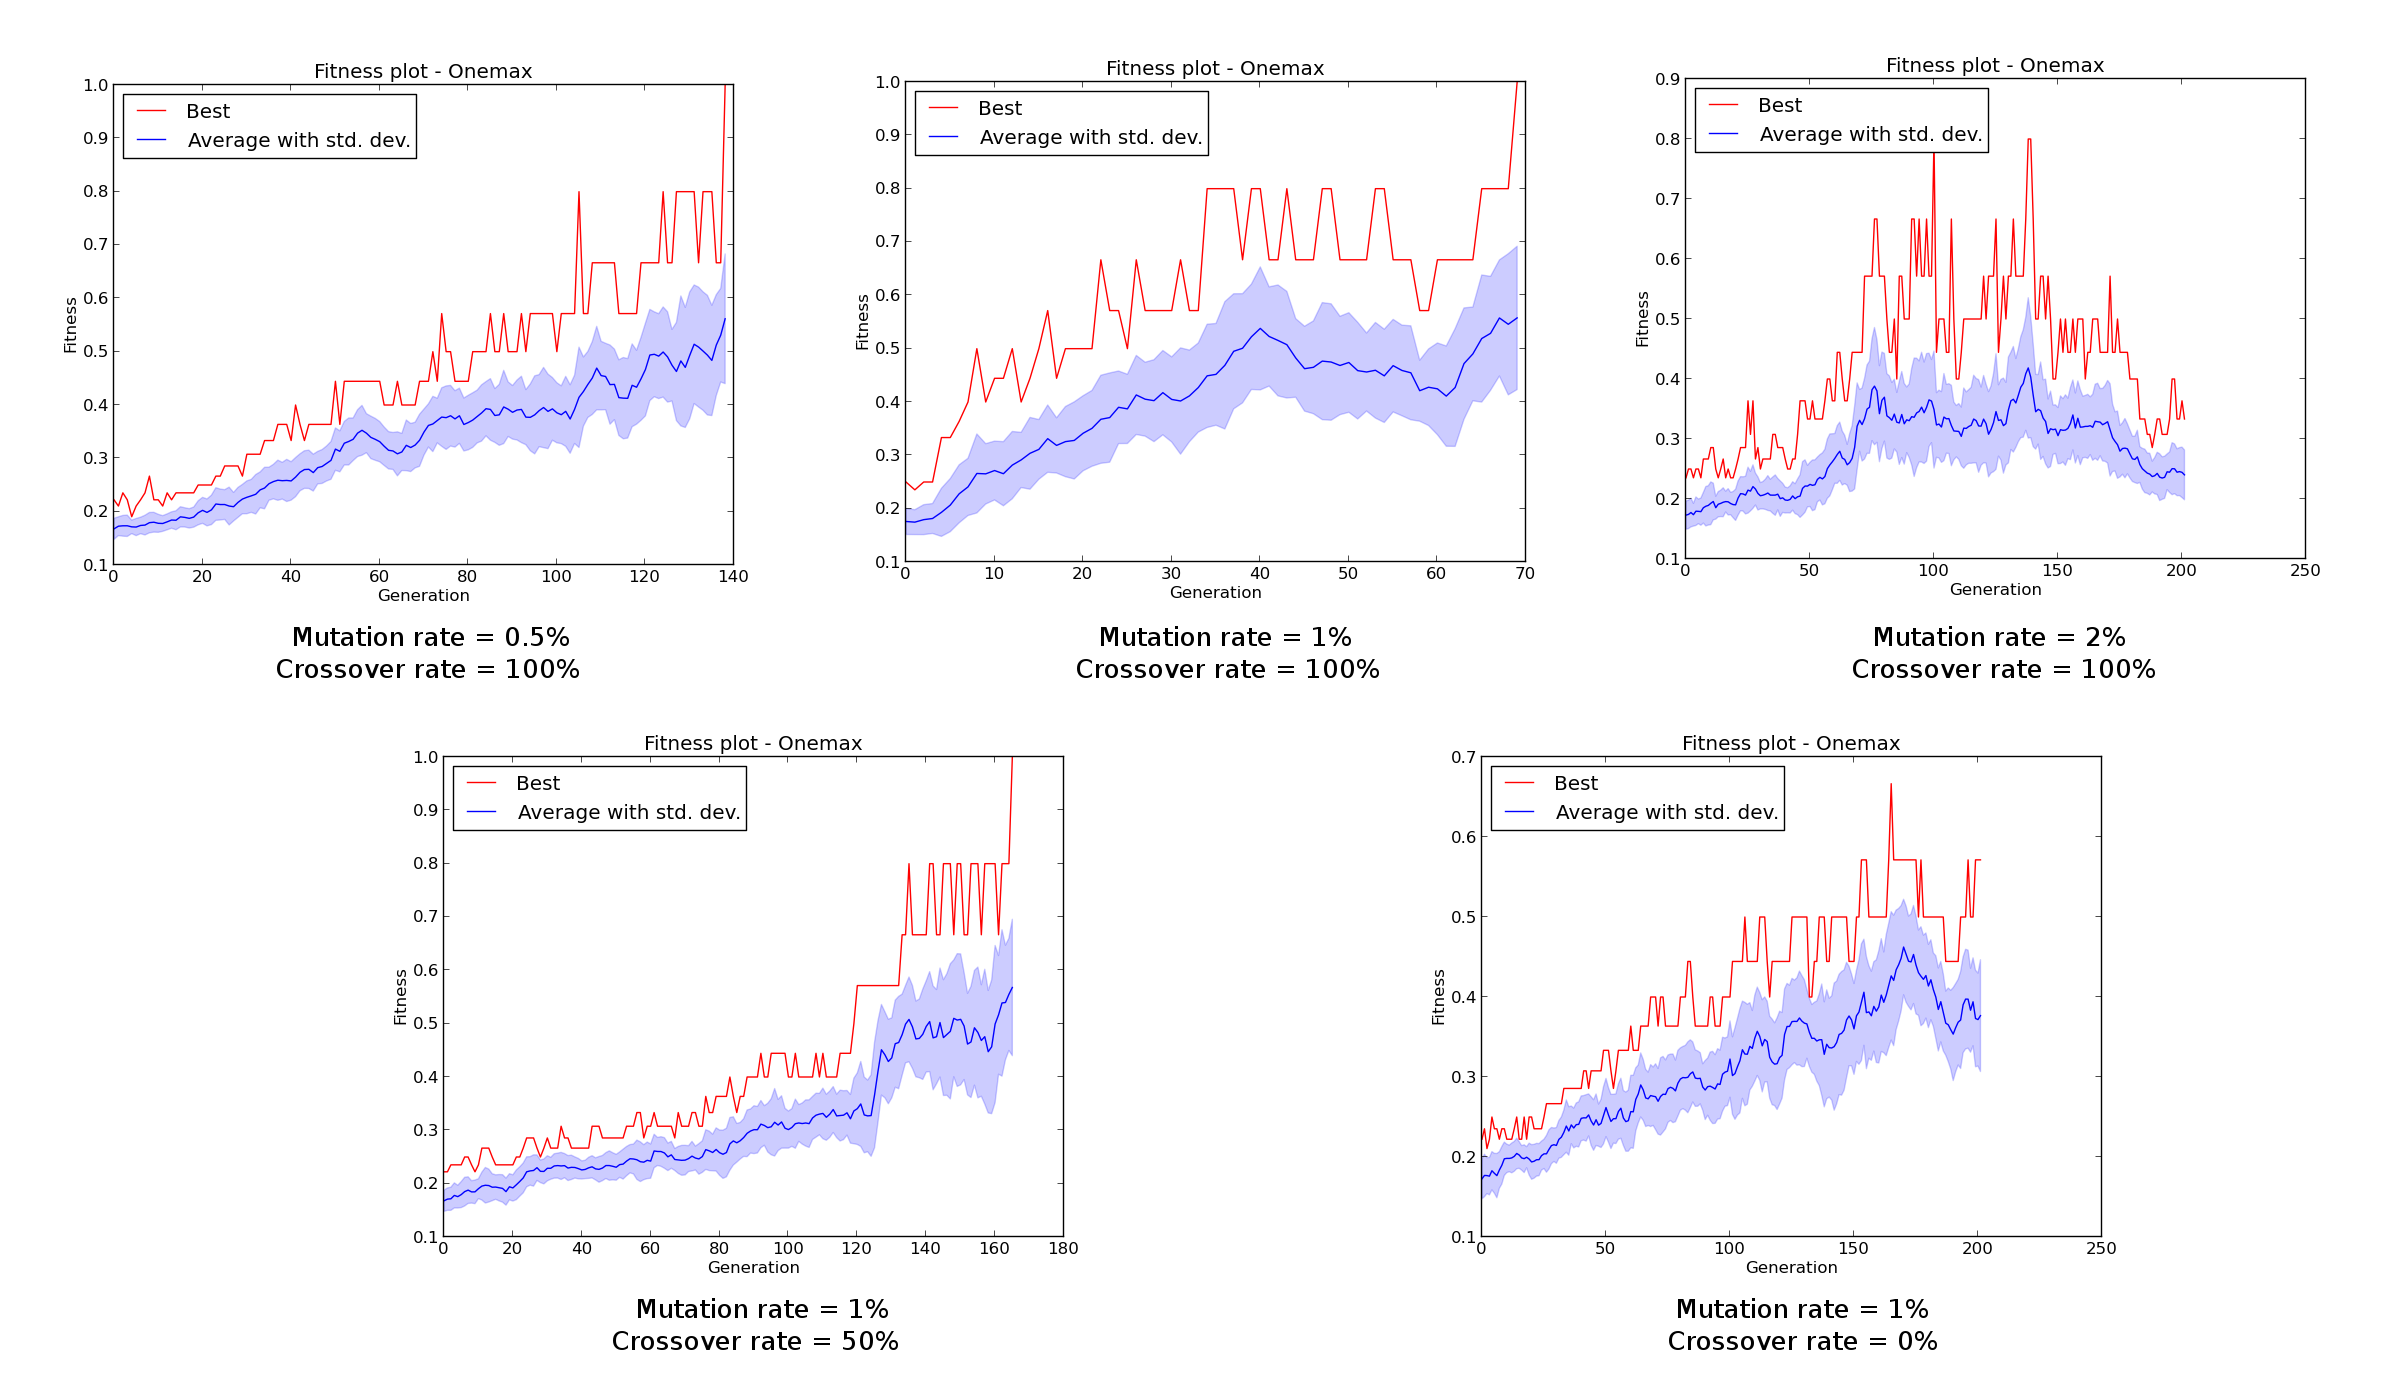
\includegraphics[width=1.2\textwidth]{graph_bundle_1}}

We see that 1\% mutation rate gets an answer quickest, so we use it for analysis of crossover rate. 2\% mutation rate and 0\% crossover rate don't get an answer at all in 200 generations, but 0\% crossover seems to be getting there. 2\% mutation just looks like a random graph.

\subsection{Parent Selection Mechanism}

% MORE PICTURES DIRECTLY TO YOUR EYES

\centerline{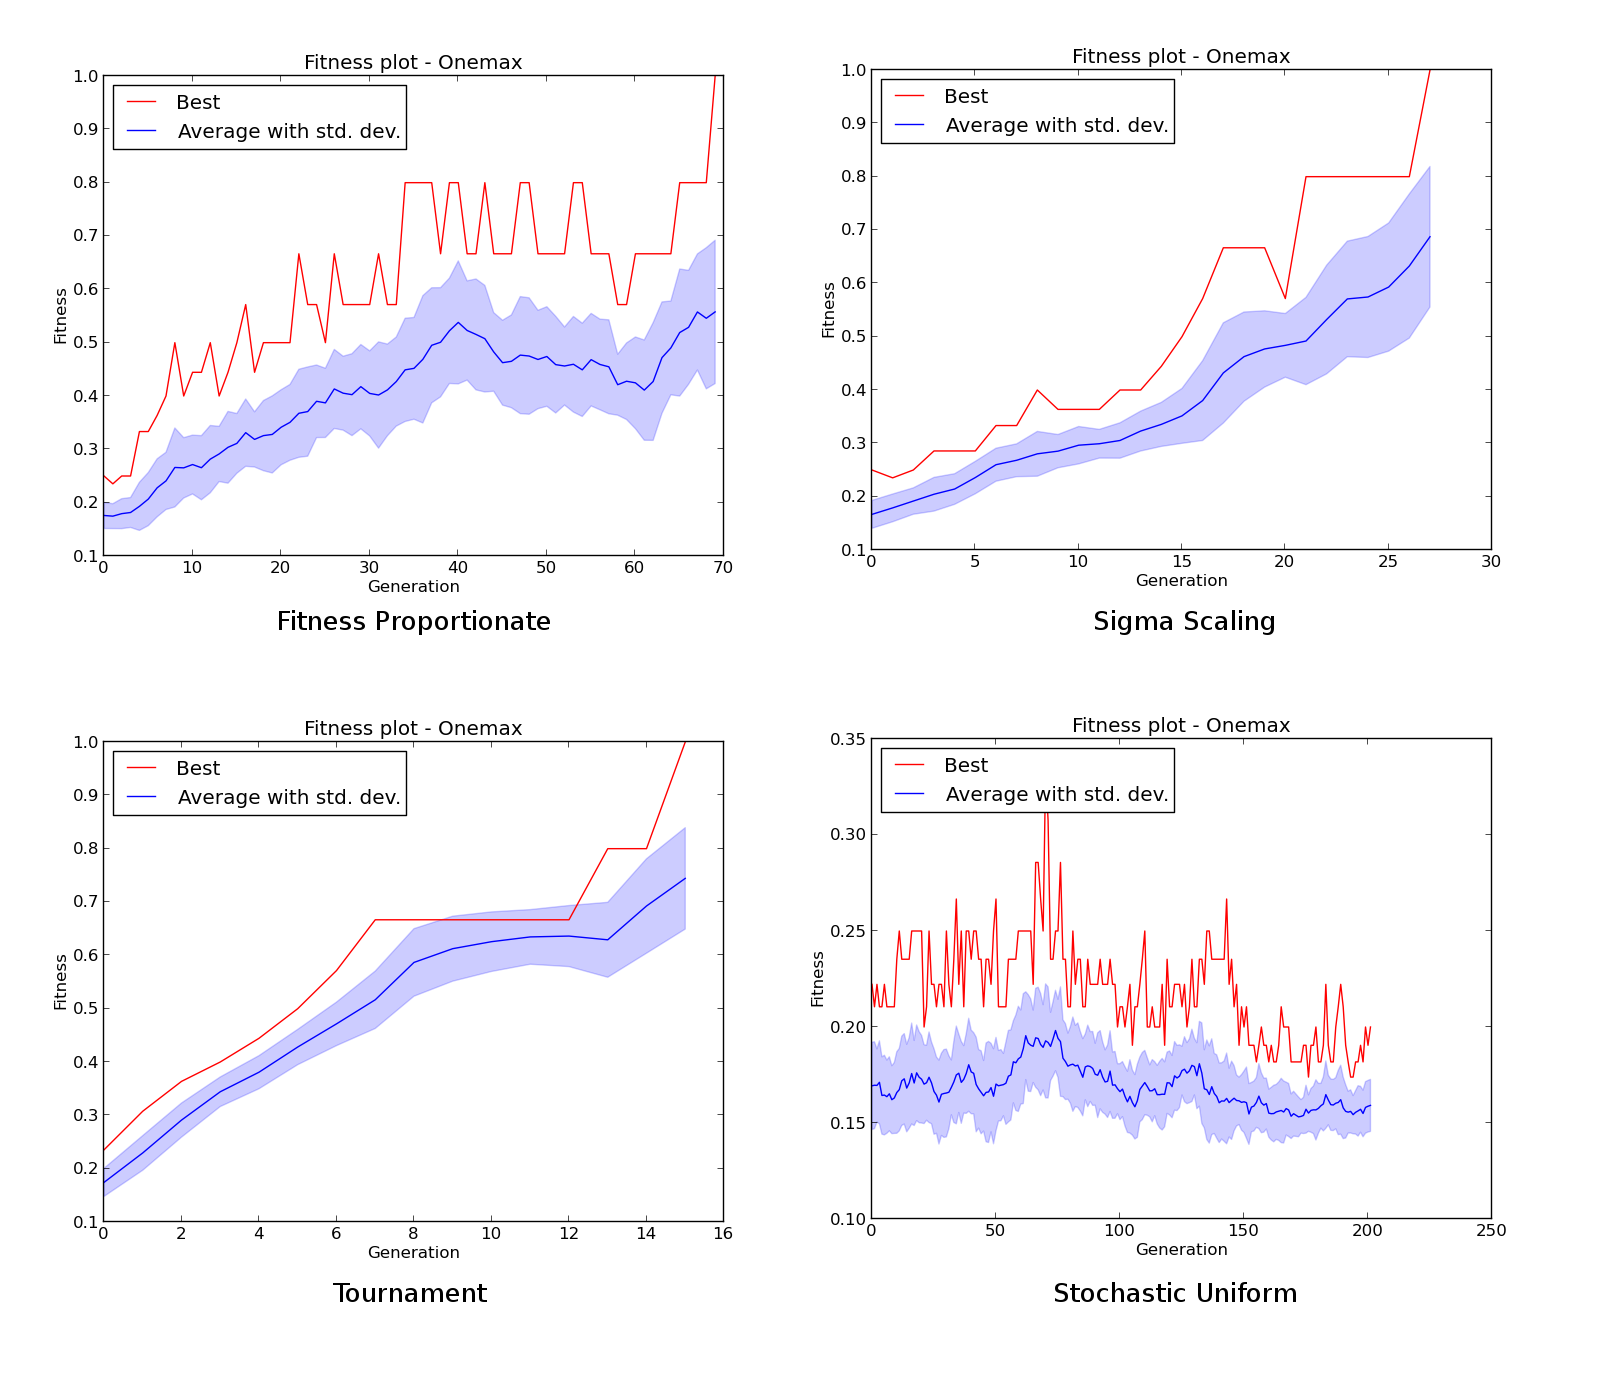
\includegraphics[width=1.2\textwidth]{graph_bundle_2}}

\begin{itemize}
\item{\textbf{Fitness Proportionate} --- Kind of slow, but it gets there.}
\item{\textbf{Sigma Scaling} --- Much better. It should also be noted that the na\"{i}ve fitness function actually works with this one, since sigma scaling sort of does the job for us.}
\item{\textbf{Tournament} --- Tournament size = 20 and $\epsilon$ = 0.1 was used. Even better results. Tournament size = Population size and $\epsilon$ = 0 would probably work even better. The reason for this is that \textsc{One-Max} has no local optima, so you lose nothing by }
\item{\textbf{Stochastic uniform} --- When paired with full generational replacement, amounts to a random search, since there is no selection pressure anywhere.}
\end{itemize}

\section{Arbitrary String Matching}
We did not expect this to impact the problem difficulty in any way, since matching a string of all ones is no different from matching any other string. One way this could have affected the difficulty is if our crossover operator had worked differently, actually putting bits from one parent's genome in another place in the child genome. But this crossover operator would have no impact on the performance of \textsc{One-Max}, and negative impact on the performance of arbitrary string matching, so it would be hard to justify. Our experiments confirmed our expectation, as can be seen from the graphs.

% OM NOM NOM TASTY PICTURES

\centerline{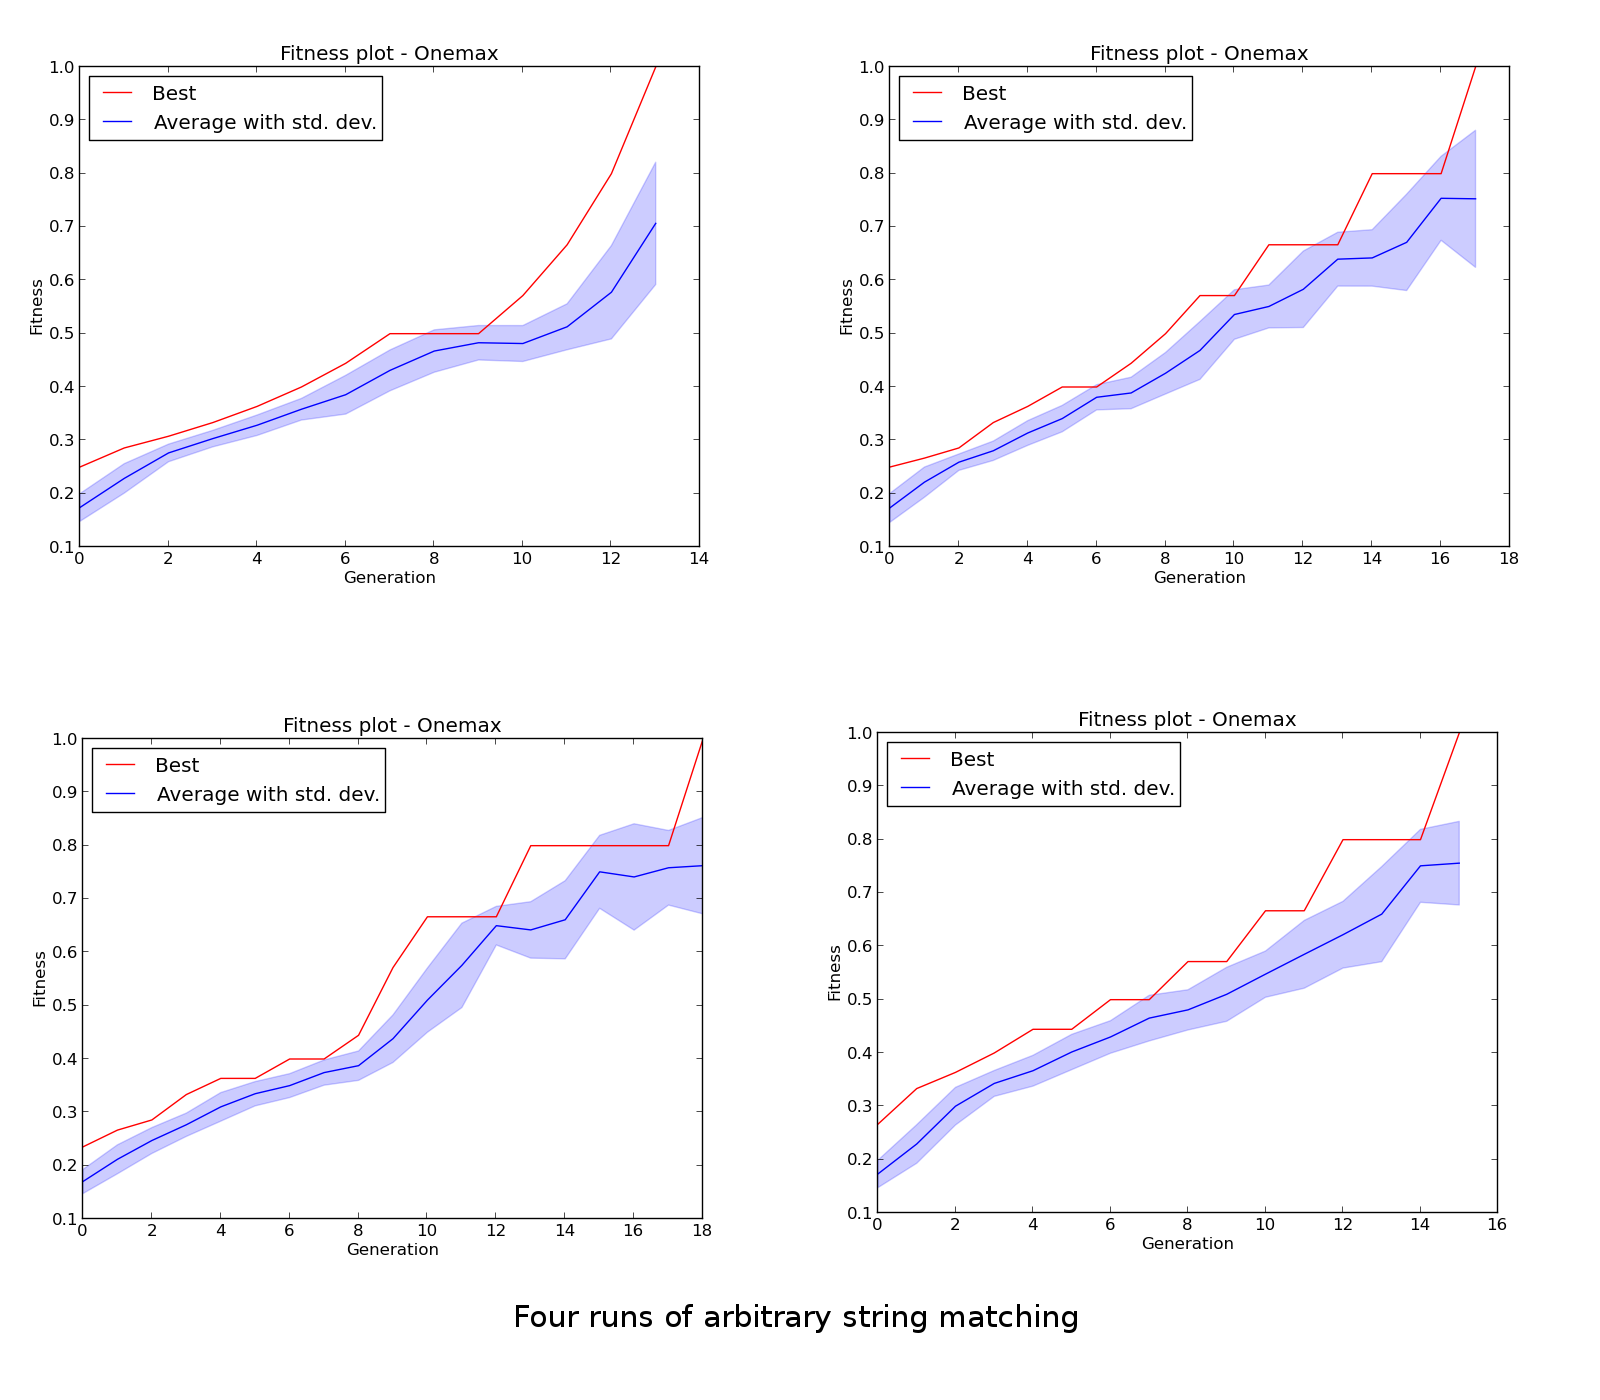
\includegraphics[width=1.1\textwidth]{graph_bundle_3}}

\end{document}
